\phantomsection
\addcontentsline{toc}{section}{Current Technology}
\section*{Current Technology}

\phantomsection
\addcontentsline{toc}{subsection}{High Performance Computing (HPC)}
\subsection*{High Performance Computing (HPC)}
High Performance Computing (HPC) marks the boundary of our current computing capabilities, and it pushes the limits of what we can achieve with classical computing. It regards the implementation of algorithms and the the hardware that they are then ran on \cite{hager2010introduction}. The most common form of HPC is the super-computer, containing thousands of compute nodes that work together to complete a task or algorithm. Modern super-computers are composed of hundreds of thousands of CPU cores and millions of GPU cores. At time of writing, \textit{Frontier} is the fastest supercomputer, performing 1.102 ExaFLOPs \cite{frontier} ($1.102\times 10^{18}$ floating point operations per second)\footnote{That is, 1.1 quintillion}, and has 591, 872 CPU cores and 7,398, 400 GPU cores.

\phantomsection
\addcontentsline{toc}{subsection}{Benefits of HPC}
\subsection*{Benefits of HPC}

\phantomsection
\addcontentsline{toc}{subsubsection}{Maturity}
\subsubsection*{Maturity}
Supercomputing systems have been around since the 1960s, with the \textit{Livermore Atomic Research Computer (LARC)}, built in 1960, being considered the oldest \cite{first_super}. Since the invention of the transistor, supercomputing technology has only increased exponentially in speed.

\begin{figure}[H]
	\centering
	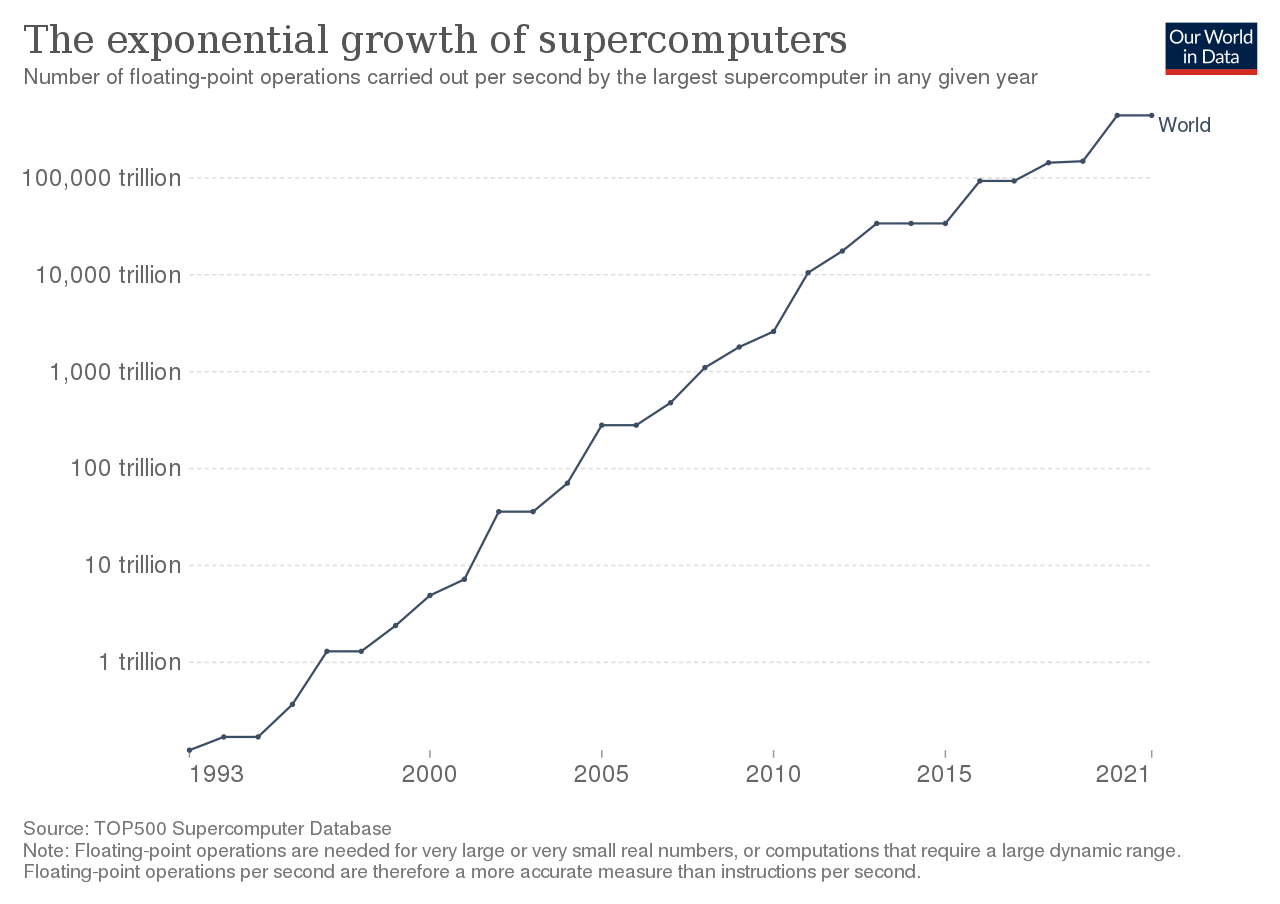
\includegraphics[width=0.7\textwidth]{Supercomputer-power-flops.png}
	\caption{Visualisation of supercomputer growth \cite{supercomputer-power-flops}}
	\label{fig:supercomputer-power-flops}
\end{figure}

This 60 year period of innovation and improvement in super-computing architectures, and processor technology has caused this technology to mature very quickly and is now used across the globe for a huge number of tasks each day. Stock markets, bank transfers, digital currencies, weather prediction and modelling, climate research are all run by HPC systems.

\phantomsection
\addcontentsline{toc}{subsubsection}{Scalability}
\subsubsection*{Scalability}
Common supercomputing architectures are now based around huge arrays of smaller computer systems, each using mostly off-the-shelf components \cite{sciences1989supercomputers}. This enables new supercomputing arrays to be set up very quickly and effectively, and at a considerably lower cost than a fully custom array would (though those systems do still exist) . It also makes them much more easier to upgrade and scale horizontally. Therefore, if a specific biological system requires more processing then it would be easy to simply add more nodes to the array and increase the capabilities of the system.

\phantomsection
\addcontentsline{toc}{subsubsection}{Ease of Setup and Maintenance}
\subsubsection*{Ease of Setup and Maintenance}
The environmental requirements of classical computers are not great. The major limitation (and cost) of HPC systems is the vast amounts of heat generated. The faster they are running, the more heat generated, requiring large amounts of cooling, either via HVAC or liquid cooling. Other than that, supercomputers can be set up anywhere there is enough space to fit it, and power for it to use.

Additionally, due to the modular nature of modern parallel systems, if a node fails, it can be easily hot-swapped out with a replacement.

\phantomsection
\addcontentsline{toc}{subsection}{Drawbacks of HPC}
\subsection*{Drawbacks of HPC}
A lot of current models for modelling biological systems are designed to model inert particles are not applicable to chemically inhomogeneous systems. The complexity of both the biological molecules and their interactions, due to the entropy of such systems. Calculating the energy levels and transfers between particles requires very detailed calculations, the number of which required scales exponentially as the number of molecules being simulated increases to fully model the system \cite{Quantum-assisted}.

Current Molecular Dynamics (MD) simulations can only simulate very small particles for very small periods of time. Using 32 CPUs to simulate a small protein, it is possible to simulate 100ns of the system in 24 hours of running the program. Therefore, to simulate that same protein with 162 ammino acids - approximately $3\times 10^{4}$ atoms - for $10\mu s$ would take 3200 CPU days \cite{MDsim}. 

Larger Molecules, for example, a ribosome, with $\approx 2.6\times 10^{6}$ atoms, being simulated for 20ns on 768 CPUs took $10^{6}$ CPU hours in 2006 \cite{Sanbonmatsu_2006}. Ribosomes produce one ammino acid every 100ms, and so to simulate the production with the same processing power, would take $10^{6}$ times longer, leading to almost 1.5 million years.

This is obviously impractical, and it is much more faster to just observe the actual system, partially due to the small time scales that biological molecules operate on and partially due to the complexity of the mathematics that underpins it.

Classical Processors are also, at their very core, linear. They can only process one instruction on one piece of data at a time. Whist running processors simultaneously can let one achieve parallel processing, there is a large amount of overhead required to coordinate each processor, which only increases as the number of processors increases.
